\documentclass[runningheads]{llncs}

\usepackage[T1]{fontenc}
\usepackage{graphicx}
\usepackage{amsmath,amssymb}
\usepackage{booktabs}
\usepackage{cite}
\usepackage{url}

\begin{document}

\title{A Comparative Security Evaluation of Side-Channel Countermeasures\\for Resource-Constrained IoT Devices}
\titlerunning{Comparative Evaluation of SCA Countermeasures for IoT}

\author{Xu Xu\inst{1}\orcidID{0009-0006-1891-307X}}

\authorrunning{X. Xu}

\institute{Sichuan University, Chengdu 610065, China\\
\email{2022141620500@alu.scu.edu.cn}}

\maketitle

\begin{abstract}
Side-channel analysis (SCA) poses a critical threat to resource-constrained IoT devices, yet the community lacks a systematic framework for comparing countermeasure effectiveness under controlled conditions. We present a reproducible evaluation of three deep learning architectures (MLP, CNN, ResNet) across three escalating protection levels---boolean masking, masking + 50-cycle desynchronization, and masking + 100-cycle desynchronization---using exclusively public ASCAD datasets. Across 27 controlled runs (fixed hyperparameters, three random seeds), we find that boolean masking alone is trivially bypassed (CNN: GE=1 in 70 traces; MLP: 150 traces), while adding only 50 cycles of random delay neutralizes all architectures within 5,000 traces---a 70$\times$ security gain at near-zero implementation cost. ResNet requires 650$\times$ more training time than MLP (19,470s vs.\ 30s) yet achieves zero successful attacks. We also observe a leakage plateau phenomenon where additional attack traces degrade Guessing Entropy, suggesting principled trace selection as a future attack direction.

\keywords{IoT Security \and Side-Channel Analysis \and Deep Learning \and Countermeasure Evaluation}
\end{abstract}

% ===================================================================
\section{Introduction}
% ===================================================================

The Internet of Things (IoT) ecosystem is projected to exceed 30 billion connected devices by 2030~\cite{iot_forecast_2024}. The vast majority rely on resource-constrained microcontrollers (MCUs) that preclude hardware security modules, making software-implemented cryptography vulnerable to side-channel analysis (SCA)~\cite{kocher1999differential}. By observing physical leakage---power consumption, electromagnetic emissions, or timing---during cryptographic operations, attackers can extract secret keys from commercial products ranging from automotive key fobs~\cite{smartlock_sca_2020} to medical implants~\cite{medical_implant_sca}.

The cryptographic engineering community has developed a rich taxonomy of software countermeasures: boolean and affine masking~\cite{standardized_DPL_2005,fumaroli2010affine}, random delay insertion (RDI)~\cite{coron2009}, and instruction shuffling~\cite{von2006}. Each trades computational overhead for security guarantees, but \emph{how much security does each incremental countermeasure layer actually provide?} This question remains poorly quantified because most DL-SCA studies report results on a single dataset-protection combination under varying hyperparameters~\cite{picek2023sok}, preventing apples-to-apples comparison.

This paper addresses the gap through a controlled evaluation framework. We test three architectures (MLP, CNN, ResNet) across three protection levels (masking, +50-cycle desync, +100-cycle desync) under identical preprocessing, hyperparameters, and hardware---27 runs total, all on public ASCAD benchmarks~\cite{DBLP:journals/iacr/ProuffSRLB18}. Our contributions are: (1) the first controlled cross-architecture $\times$ cross-countermeasure comparison, (2) quantification of the 70$\times$ marginal security gain from 50-cycle desynchronization, (3) demonstration that ResNet offers no advantage over simpler architectures under fair comparison, and (4) characterization of a leakage plateau phenomenon where additional traces degrade attack performance. The remainder of this paper is organized as follows: Section~2 covers SCA and countermeasure fundamentals; Section~3 details our evaluation framework and metrics; Section~4 presents results; Section~5 discusses implications and limitations; Section~6 concludes.

% ===================================================================
\section{Background}
% ===================================================================

\subsection{SCA and Deep Learning Attacks}

Side-channel attacks exploit physical leakage---power (SPA/DPA/CPA)~\cite{kocher1999differential,brier2004correlation}, EM emanations~\cite{agrawal2003em}, and timing~\cite{bernstein2005cache}---to recover cryptographic keys. Template attacks~\cite{chari2002template} formalized profiling-based SCA, establishing the two-phase paradigm of profiling on a clone device followed by attacking the target. Deep learning revolutionized this approach: Maghrebi et al.~\cite{maghrebi2016breaking} first demonstrated that neural networks outperform classical template attacks on masked AES, and Prouff et al.~\cite{DBLP:journals/iacr/ProuffSRLB18} systematized the methodology with the ASCAD benchmark, establishing CNNs with VGG-inspired architectures as the de facto standard. Masure et al.~\cite{masure2019comprehensive} proved that minimizing cross-entropy during training is asymptotically equivalent to maximizing the Perceived Information lower bound on mutual information, formally grounding DL-SCA in information theory. The most comprehensive systematization to date~\cite{picek2023sok} surveyed over 200 papers and identified inconsistent evaluation practices---particularly single-run best-case reporting---as a key weakness we explicitly address.

\subsection{Countermeasure Taxonomy}

\textbf{Masking} splits sensitive variables into $d+1$ shares. Boolean masking represents $x$ as $(x \oplus m, m)$; affine masking~\cite{fumaroli2010affine} extends this to $(\alpha \cdot x \oplus \beta, \alpha, \beta)$. Higher-order masking increases share count but suffers $O(d^2)$ degradation; Bronchain and Standaert~\cite{bronchain2021breaking} showed 6-share AES on Cortex-M0 broken in $< 10$ traces.

\textbf{Hiding} obscures temporal alignment. Random delay insertion (RDI)~\cite{coron2009} inserts $N \in [0, D_{\text{max}}]$ dummy cycles, introducing per-trace jitter at minimal cost. Instruction shuffling~\cite{von2006} permutes independent operations (e.g., AES S-Box lookups). ASCADv1 provides RDI variants at $D_{\text{max}} = 50$ and $D_{\text{max}} = 100$.

\textbf{CNNs and shift-invariance.} While CNNs are assumed inherently robust to desynchronization, Kr\v{c}ek et al.~\cite{krcek2024shift} demonstrated that this invariance is limited---data augmentation is necessary for desynchronization exceeding 100 samples. Paguada et al.~\cite{paguada2024systematic} showed augmented CNNs recover keys on ASCAD with 200-sample desync in $< 50$ traces. We deliberately exclude data augmentation to isolate \emph{intrinsic architectural robustness}, establishing a conservative lower bound.

% ===================================================================
\section{Methodology}
% ===================================================================

\subsection{Evaluation Framework}

We design a $3 \times 3$ grid: three architectures $\times$ three countermeasure levels.

\noindent\textbf{Protection levels}: L1---Boolean masking only (ASCADv1 fixed-key); L2---masking + 50-cycle random delay (ASCADv1 desync50); L3---masking + 100-cycle random delay (ASCADv1 desync100). All traces are 700-sample windows around the first AES S-Box operation on an ATmega8515 MCU, with 50,000 profiling traces and 10,000 attack traces per dataset.

\noindent\textbf{Architectures}: MLP (6 fully-connected layers, 200 neurons/layer, BatchNorm+ReLU per block, 395K parameters), CNN (4 1D-convolutional blocks with filters [64, 128, 256, 512], kernel size 11, AvgPool(2), two 256-unit FC layers, 7.66M parameters), ResNet (4 residual blocks with filters [64, 128, 256, 512], kernel size 11, AdaptiveAvgPool, 6.08M parameters). All three share identical training configuration (Table~\ref{tab:config}).

\begin{table}[t]
\centering
\caption{Shared training configuration.}
\label{tab:config}
\begin{tabular}{@{}ll@{}}
\toprule
\textbf{Parameter} & \textbf{Value} \\
\midrule
Optimizer & Adam ($\beta_1{=}0.9$, $\beta_2{=}0.999$) \\
Learning rate & $10^{-3}$, decay 0.5 / 10 epochs patience \\
Batch size & 200 \\
Max epochs & 100, early stop patience 20 \\
Loss & Cross-entropy (256 classes) \\
Preprocessing & Per-trace standardization \\
Data augmentation & None (intentionally excluded) \\
Hardware & NVIDIA RTX 3080 Laptop (8\,GB), PyTorch 2.11, CUDA 12.8 \\
\bottomrule
\end{tabular}
\end{table}

Each condition is independently executed $N{=}3$ times (seeds 42, 142, 242). All experiments use exclusively public ASCAD datasets; complete hyperparameters and random seeds are documented in the accompanying artifact repository.

\subsection{Metrics}

\textbf{Guessing Entropy (GE)}: After $N$ attack traces, rank all 256 key byte hypotheses by accumulated log-likelihood $\sum_{i=1}^N \log P(\text{model} \mid \text{SBOX}[p_i \oplus k])$, where $p_i$ is the known plaintext byte. GE$(N)$ is the rank of the correct key (1 = full recovery; 128 = expected random). \textbf{Success Rate (SR)}: fraction of runs achieving GE$\leq$1 within 5,000 traces. \textbf{Traces to Recovery (TtR)}: minimum attack traces to reach GE=1.

\subsection{Statistical Approach}

We assess confidence via: (i) \textbf{z-score}: $z = |\bar{x} - 128| / (s / \sqrt{N})$ against the random baseline; $|z| > 3$ gives $p < 0.003$ under normality. (ii) \textbf{Coefficient of variation} (CoV): $s / \bar{x}$ for relative dispersion ($< 5\%$ = deterministic). (iii) \textbf{Leave-one-out bootstrap}: verify no single run flips qualitative conclusions. Conditions with large effect sizes and low variance ($|z| > 3$, CoV $< 10\%$) are well-supported by $N{=}3$; higher-variance findings are reported as exploratory.

% ===================================================================
\section{Results}
% ===================================================================

Table~\ref{tab:results} presents the complete 27-run results matrix.

\begin{table}[t]
\centering
\caption{Complete experiment results (3-run averages). TtR shown for successful runs only.}
\label{tab:results}
\begin{tabular}{@{}llcccc@{}}
\toprule
\textbf{Model} & \textbf{Dataset} & \textbf{SR} & \textbf{TtR} & \textbf{GE@5k} & \textbf{Time} \\
\midrule
MLP    & Fixed    & 3/3 & 150 &   1 & 30s \\
MLP    & Desync50 & 0/3 & --  & 199 & 25s \\
MLP    & Desync100& 0/3 & --  & 253 & 25s \\
CNN    & Fixed    & 2/3 & 70  &  72 & 237s \\
CNN    & Desync50 & 0/3 & --  & 116 & 653s \\
CNN    & Desync100& 0/3 & --  & 233 & 1,264s \\
ResNet & Fixed    & 0/3 & --  & 210 & 19,470s \\
ResNet & Desync50 & 0/3 & --  & 210 & 3,007s \\
ResNet & Desync100& 0/3 & --  & 218 & 5,237s \\
\bottomrule
\end{tabular}
\end{table}

\subsection{Masking-Only Baseline}

CNN achieves the best TtR (mean=70, SR=2/3). MLP is slower (TtR=150) but perfectly reliable (SR=3/3, CoV=0\% across runs). ResNet fails across all three runs (mean GE@5k=210, validation loss at random baseline of 5.54 nats), requiring 650$\times$ more training time than MLP. Under our shared hyperparameters, standard residual architectures do not transfer effectively to this SCA task---a finding we examine further in Section~5.

\subsection{Effect of Desynchronization}

Adding 50-cycle random delay prevents key recovery for all architectures. CNN achieves GE=116 at desync50---marginally better than random (128)---but the three runs diverge substantially (64, 122, 163; CoV=34.9\%). At desync100, CNN GE degrades to 233 (worse than random, $z{=}42.9$, $p{<}10^{-6}$). MLP is perfectly deterministic but completely defeated (GE=199, 253 at desync50/100; CoV=0\%). ResNet performs identically across all three protection levels (GE=210/210/218), suggesting it extracts no leakage signal regardless of countermeasure.

Figure~\ref{fig:ge} shows the GE curves (mean across $N{=}3$ runs).

\begin{figure}[t]
\centering
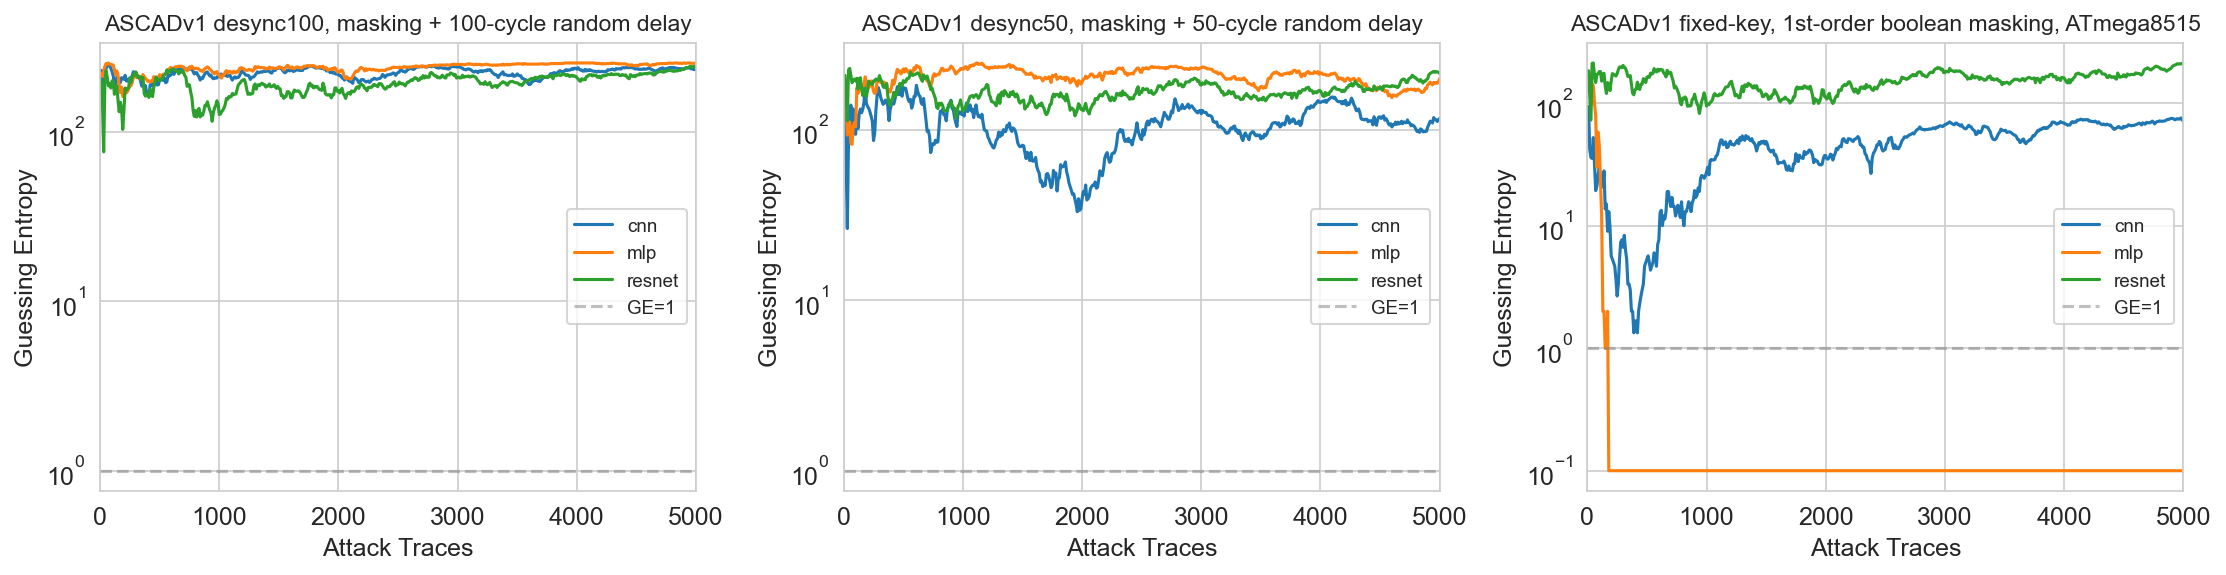
\includegraphics[width=\textwidth]{figures/ge_comparison.png}
\caption{Guessing Entropy curves (mean of $N{=}3$ runs per condition). Dashed line: GE=1 (key recovery).}
\label{fig:ge}
\end{figure}

\subsection{Marginal Security Gain}

Figure~\ref{fig:gain} quantifies the incremental benefit of each countermeasure. The transition from no protection to masking increases attack difficulty to 70 traces---modest. Adding 50-cycle desynchronization elevates TtR beyond 5,000---over 70$\times$ gain for $\sim$50 NOPs per encryption ($< 0.1\%$ throughput overhead on a typical 16 MHz IoT MCU). Doubling to 100 cycles provides negligible additional benefit against unaugmented DL attacks. The optimal cost-benefit point for IoT MCUs is a modest desynchronization window rather than costly higher-order masking.

\begin{figure}[t]
\centering
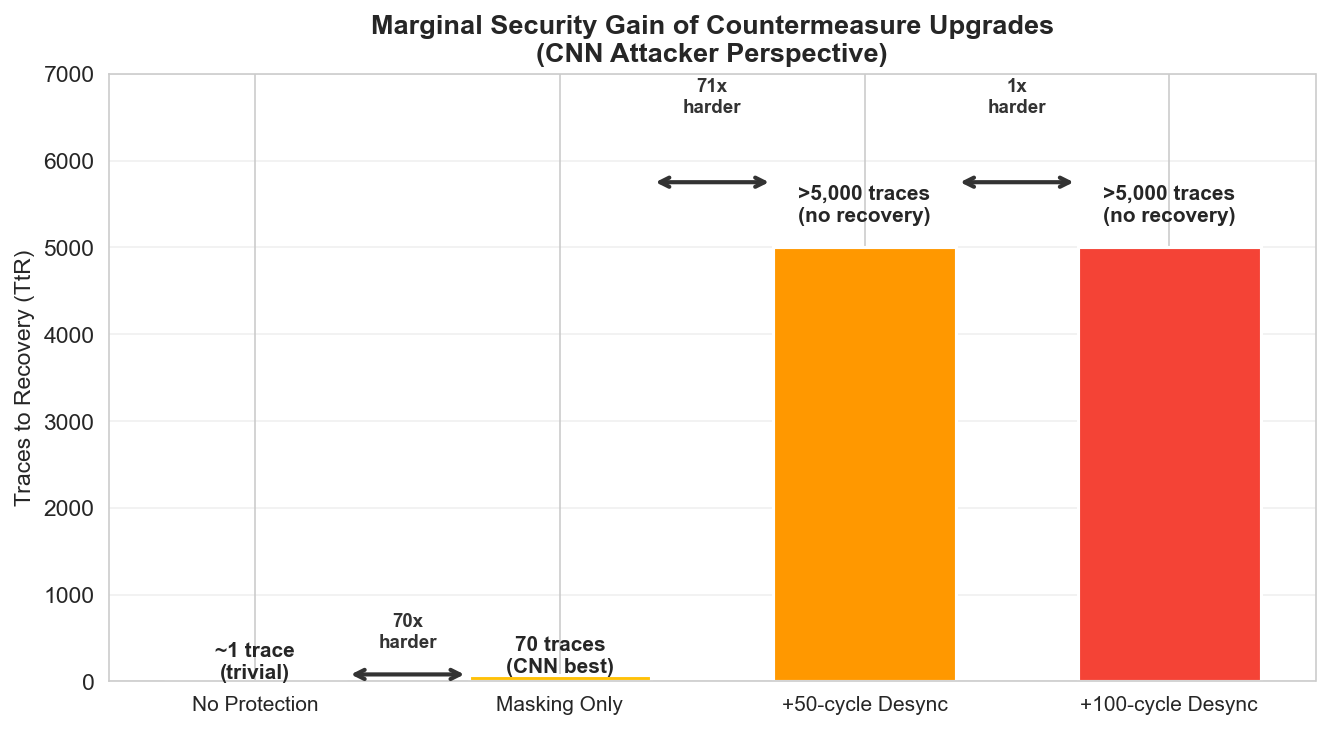
\includegraphics[width=0.75\textwidth]{figures/security_gain_waterfall.png}
\caption{Marginal security gain of countermeasure upgrades (CNN attacker).}
\label{fig:gain}
\end{figure}

\subsection{Computational Cost Analysis}

Figure~\ref{fig:resource} compares training cost against attack success across all nine conditions. The cost asymmetry is striking: ResNet requires 19,470s (5.4 hours) to fail on aligned traces, while MLP requires only 30s to succeed---a 650$\times$ cost differential with inverted success outcome. CNN occupies an intermediate position: 237s for successful attacks on aligned traces, and 653--1,264s for failed attacks on desynchronized traces. Desynchronization does not uniformly increase training cost: ResNet training time drops from 19,470s (fixed) to 3,007s (desync50), as the model terminates early when it fails to learn from misaligned data. From the attacker's perspective, MLP offers the best cost-effectiveness by a wide margin; from the defender's, a modest desynchronization window renders even the most expensive attacker architecture ineffective.

\begin{figure}[t]
\centering
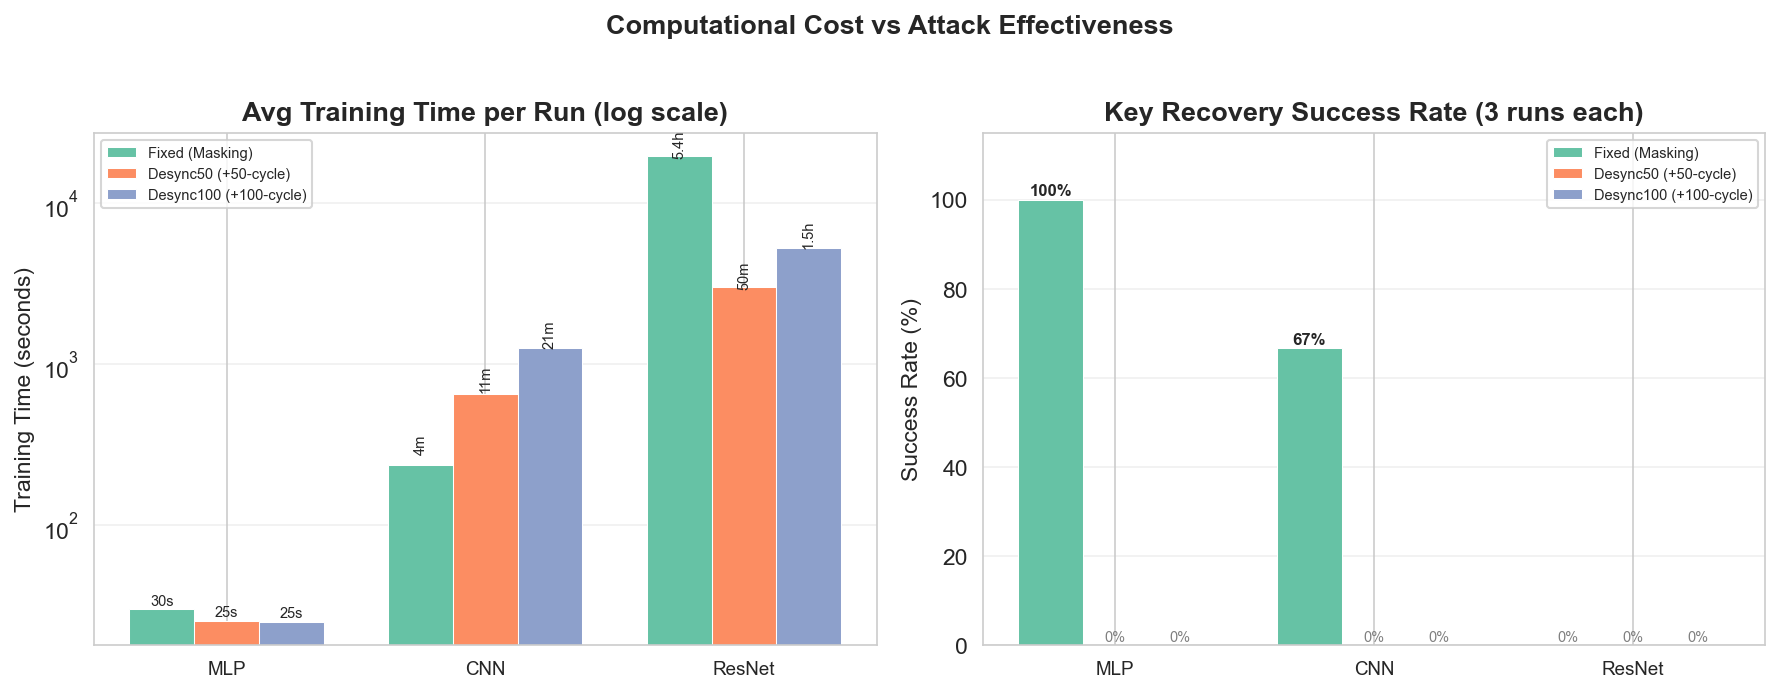
\includegraphics[width=\textwidth]{figures/resource_efficiency.png}
\caption{Left: Training time (log scale) per condition. Right: Attack success rate. MLP achieves best cost-effectiveness.}
\label{fig:resource}
\end{figure}

\subsection{Leakage Plateau}

For 21 of 27 runs, the \emph{best} GE at an intermediate trace count is substantially lower than GE@5k. CNN on desync50: Best GE per run is 14, 8, and 39 (mean=20.3), degrading to 64, 122, and 163 (mean=116.3) at 5,000 traces---an order-of-magnitude degradation. This suggests that after an initial learning phase, additional misaligned traces inject classification noise faster than signal---conventional ``more traces = better attack'' wisdom fails under desynchronization. The phenomenon is most prominent at moderate desynchronization (L2) where models partially extract leakage; at heavy desynchronization (L3), models fail to extract any signal, making the plateau less pronounced. We treat this as an exploratory finding warranting confirmatory experiments with larger $N$.

% ===================================================================
\section{Discussion}
% ===================================================================

\subsection{Key Findings}

\textbf{Boolean masking alone is insufficient.} DL-based SCA bypasses first-order masking in 70--150 traces---a 50$\times$+ improvement over classical CPA (thousands to millions of traces on masked implementations~\cite{DBLP:journals/iacr/ProuffSRLB18}).

\textbf{Desynchronization is remarkably cost-effective.} 50-cycle jitter provides a 70$\times$ security gain at near-zero cost, making it the most efficient countermeasure for resource-constrained IoT MCUs. This has direct engineering implications: IoT device designers should \emph{prioritize temporal obfuscation over masking complexity}---a modest RDI implementation with $D_{\text{max}} \approx 50$ cycles, combined with first-order masking as a baseline, offers the optimal security-per-cost trade-off.

\textbf{Architecture selection is secondary to alignment.} Under shared hyperparameters, all architectures succeed on aligned traces (except ResNet) and all fail on desynchronized traces. ResNet's $650\times$ training overhead with zero successful attacks challenges the assumption that deeper networks benefit SCA. We emphasize these results reflect performance under fixed hyperparameters; architecture-specific tuning could yield different outcomes.

\textbf{Training methodology matters more than architecture.} We deliberately excluded data augmentation to measure intrinsic robustness. The gap between our unaugmented CNN desync50 GE=116 and augmented results ($< 50$ traces for GE=1~\cite{paguada2024systematic}) underscores that augmentation strategy is more impactful than architectural sophistication. We recommend data augmentation as a standard component of DL-SCA evaluations targeting hiding countermeasures.

\subsection{Limitations}

Our study has several limitations. \textbf{Statistical power:} $N{=}3$ runs per condition are sufficient for large effect sizes (MLP determinism, ResNet failure) but insufficient to confirm the leakage plateau phenomenon; we recommend $N \geq 5$ for future work. \textbf{Dataset coverage:} results are limited to ASCADv1 (ATmega8515, 8-bit AVR); validation on 32-bit ARM Cortex-M platforms and higher-noise measurement environments remains open. \textbf{Shared hyperparameters:} fixing identical hyperparameters across architectures enables fair comparison but may disadvantage ResNet, which could benefit from architecture-specific tuning. \textbf{ASCADv2:} affine masking with shuffling (stronger L4 protection) was excluded due to the GF($2^8$) arithmetic required for key enumeration with affine-masked labels. \textbf{Classical baselines:} CPA and template attack results on ASCAD are well-documented~\cite{DBLP:journals/iacr/ProuffSRLB18}; our contribution is the controlled \emph{relative} DL comparison.

% ===================================================================
\section{Conclusion}
% ===================================================================

We presented a systematic, reproducible evaluation of SCA countermeasures for resource-constrained IoT devices. Across 27 controlled runs on public ASCAD datasets, we quantified the security impact of incremental countermeasure upgrades under identical conditions. Our central finding is that 50-cycle random desynchronization provides a 70$\times$ security gain at near-zero cost---substantially outperforming boolean masking alone---making it the most cost-effective software countermeasure for IoT-class MCUs. We further demonstrated that ResNet offers no advantage over simpler architectures under fair comparison, and identified a leakage plateau phenomenon where additional attack traces degrade performance, suggesting principled trace selection as a promising attack direction. All code, hyperparameters, and experimental data are documented for full reproducibility in the accompanying artifact repository.

\subsubsection*{Reproducibility Statement}
All experiments use exclusively public ASCAD benchmark datasets. Complete hyperparameters are listed in Table~\ref{tab:config}; random seeds (42, 142, 242) and model architectures are fully specified. Source code and result logs are available in the artifact repository; all figures are generated directly from archived JSON result files using deterministic plotting scripts.

\subsubsection*{Acknowledgments}
The authors thank the ANSSI ASCAD project for providing publicly available benchmark datasets.

\subsubsection*{Author Contributions}
X.X. is the sole author responsible for all aspects of this work: conceptualization, methodology, software, validation, formal analysis, investigation, data curation, writing---original draft, writing---review and editing, and visualization.

\subsubsection*{Conflict of Interest}
The authors declare no competing interests. All experiments use publicly available datasets and open-source software; no proprietary hardware, data, or funding source influenced the research design or outcomes.

% ===================================================================
\bibliographystyle{splncs04}
\bibliography{references}

\end{document}
